%************************************************
\chapter{The Taste Experiment}
%************************************************
\section{Objective}
To find out if there exists a relation between the number of papillae and a specific compound tasting ability of humans from varied geographical locations, using a small sample size.

\section{Requirements}
	\begin{enumerate}
		\item Blue Food Colouring
		\item Tooth picks
		\item PROP Test Paper (6-n-propylthiouracil)
		\item White Paper
		\item A pair of Scissors, pencil and a ruler
	\end{enumerate}

\section{Background Theory}
	Certain compounds are bitter to some humans and completely tasteless to others. The bitterness has two levels, which we call super tasters and tasters. The compound used initially for this analysis was PCT and it was hypothesized that there're two alleles that control this, like a typical mandelian system, with the dominant homozygote as super taster, heterozygote as taster and the recessive homozygote as non-taster.
	\par
	Eventually when the PTC gene was located, it was found that it encodes for one of the 25 bitter taste receptor proteins present in the taste buds of human tongue. There are 3 different kinds of Single Nucleotide Polymorphisms which result in 5 haplotypes. The two most common are \emph{PAV}, a major taster haplotype and \emph{AVI}, a major non-taster haplotype. When both are PAV, the individual is very likely a super taster and when both are AVI, the individual's very likely to be a non-taster.
	\par
	Here, we try to see if there's a relation between the number of receptors and the tasting ability. According to prior research, density usually helps tasting. The method to identify the density, harnesses the fact that the filiform papillae stain dark blue (filiform are those that do NOT contain any taste buds) and the fungiform papillae (fungiform papillae contain taste buds) stain lighter and can be easily distinguished under sufficient light.

\section{Statistical Analysis}
	We make a very simple assumption here. We assume that for the total population, the number of papillae is independent of individuals being tasters or non-tasters and that the distribution is normal. This is our Null hypothesis. If there is a relation between the papillae count and the tasting ability, then the Null hypothesis must get rejected after the analysis. Now, assuming the Null hypothesis to be true, what we have is two means and two variances, one for the tasters and other for the non-tasters. In accordance with the hypothesis, these are simply two samples taken from the aforesaid population. If we now take the difference of these means, then it's likely to be close to zero, if the hypothesis is true that is. We now just need a method to quantify how close, rather how far must these means be so that we can reject the Null hypothesis. Since the sample size is extremely small we use student's T distribution which depends on only the the degrees of freedom of the system being analysed. If we can relate our means and variances with this distribution, it becomes simply a matter of looking up values to find the probability of their occurrence, assuming the Null hypothesis to be true. We now define a less than $5\%$ probability of occurrence to mean that the \emph{means} are too different to belong to the aforesaid population, and thus the null hypothesis must be rejected.
	\par
	That might sound a wee-bit complicated, but practically here's what needs to be done. We've found experimentally, $m_1$, $m_2$, $s_1$, $s_2$, $n_1$ and $n_2$, which are means, variances and degrees of freedom respectively. We find the $t$ value using the following equation
	\begin{equation}
		t=\frac{m_1 - m_2}{\sqrt{\frac{s_1^2}{N_1} + \frac{s_2^2}{N_2}}}
	\end{equation}
	Also, we find the degrees of freedom, given by
	\begin{equation}
		df = (N_1 -1) + (N_2 -1) = (N_1 + N_2 -2)
	\end{equation}
	Now all we have to do is look up the value in a t-table corresponding to $0.025$ and $df$ as calculated. If $t_\text{calculated}>t_\text{table}$, then the Null hypothesis is rejected. Else, the null hypothesis can not be rejected.
	\par
	We used $0.025$ for the t-table instead of $0.5$ simply because we're assuming our distribution to be symmetric and thus $0.025$ on both sides adds up to a $5\%$ probability, consistent with our previous benchmark. What we've performed is a two tailed test (name should now be obvious).

\section{Procedure}
	\begin{enumerate}
		\item Took a PROP taste paper and placed it on the tongue to identify each individual as a super taster, taster or non-taster.
		\item Dabbed some food colour on a toothpick and swabbed the tongue with it, till an appropriately distinguishable set of spots were visible. 
		\item Placed a paper with 1 $cm^2$ area on the tongue. The tongue was held static (teeth were used) while a person counted the fungiform papillae on the tongue.
		\item This was repeated for another position on the tongue. 
		\item Both these counts were recorded.
		\item Both numbers were recorded and means and variances calculated as described earlier.
	\end{enumerate}

\section{Observations and Results}
	Observations and calculations are given in \autoref{taste}. The t value was found to be $0.1044$ which is much smaller than $t_{df=15, \alpha=0.025}=2.080$ as given in \autoref{t_table}, thus the Null hypothesis can NOT be rejected.

	\begin{figure}[bth]
		\begin{center}
			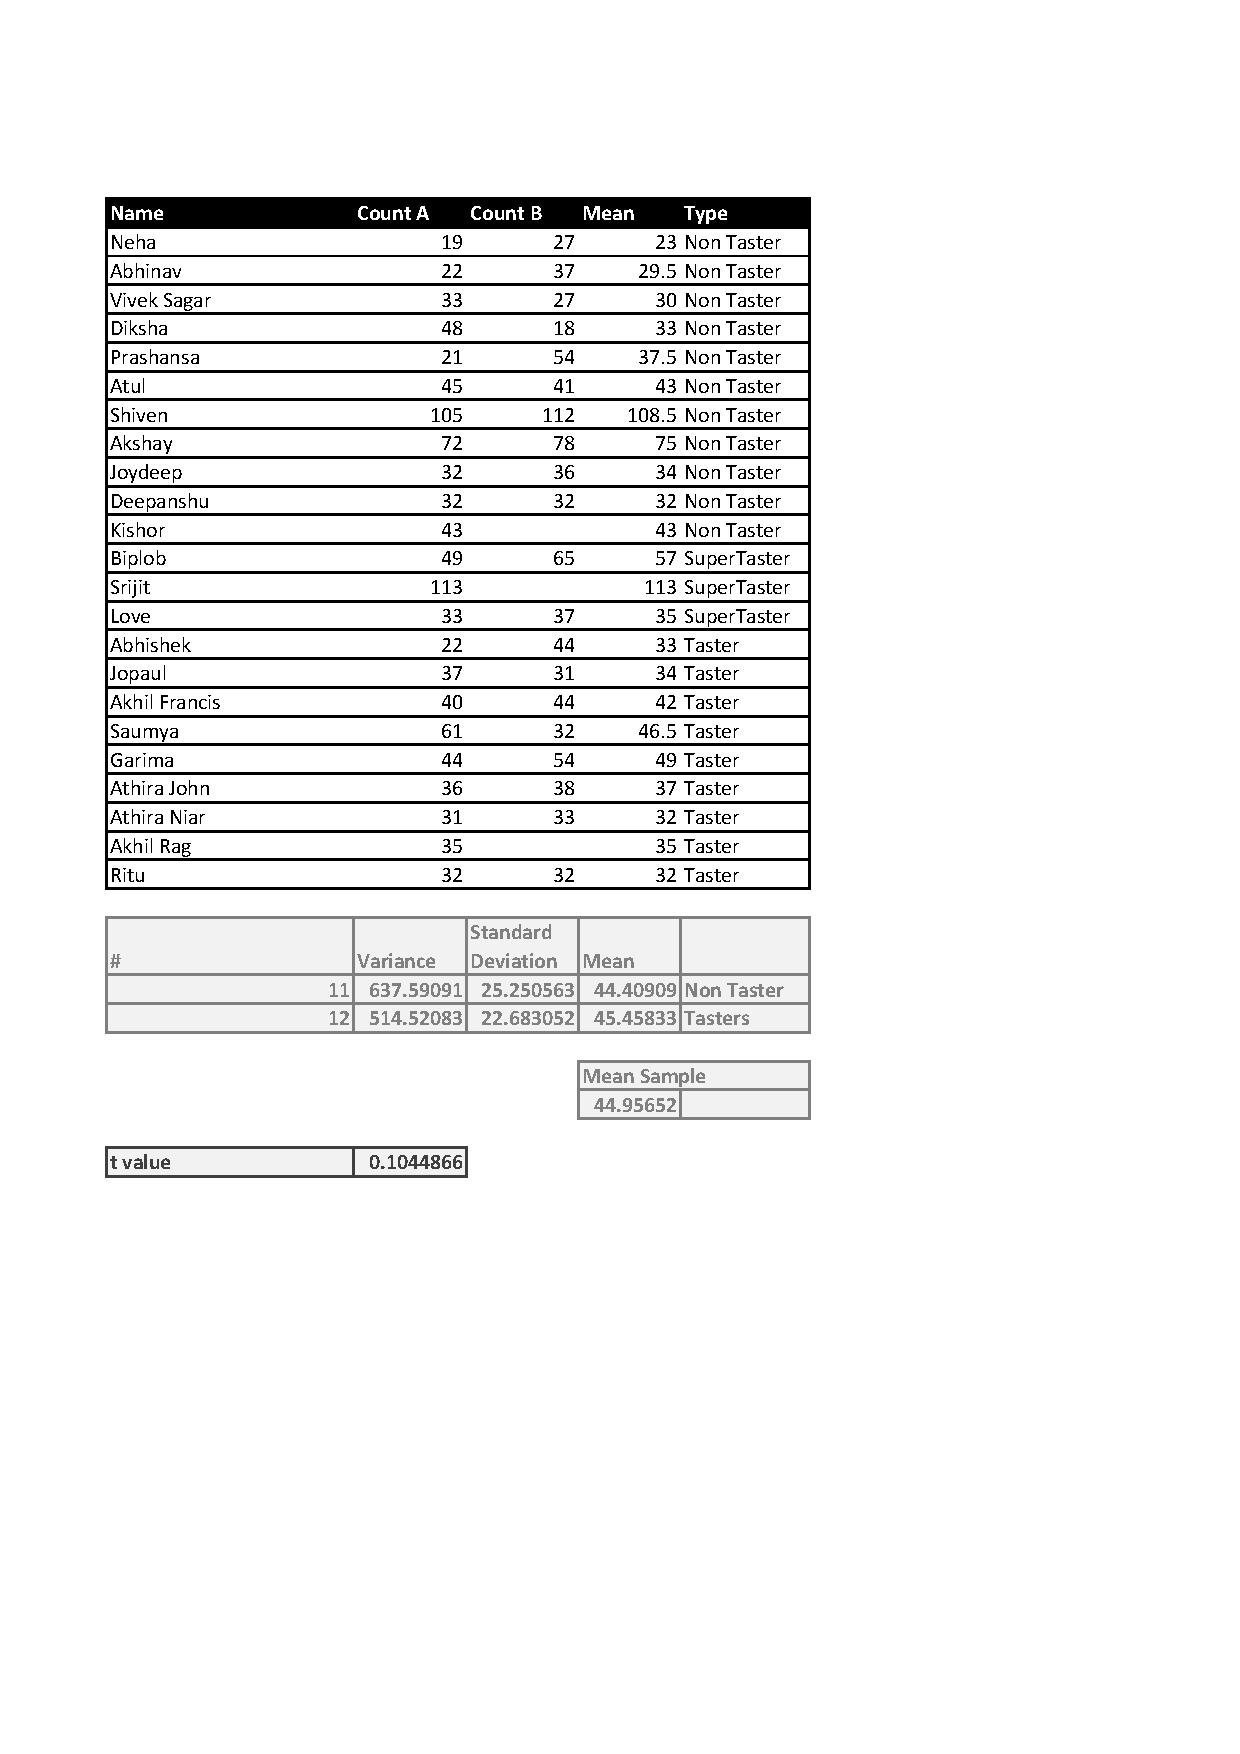
\includegraphics[width=1.5\linewidth]{gfx/final_taste}
		\end{center}
	\caption[Observations and Calculations]{Observations and Calculations}
	\label{taste}
	\end{figure}	

	\begin{figure}[bth]
		\begin{center}
			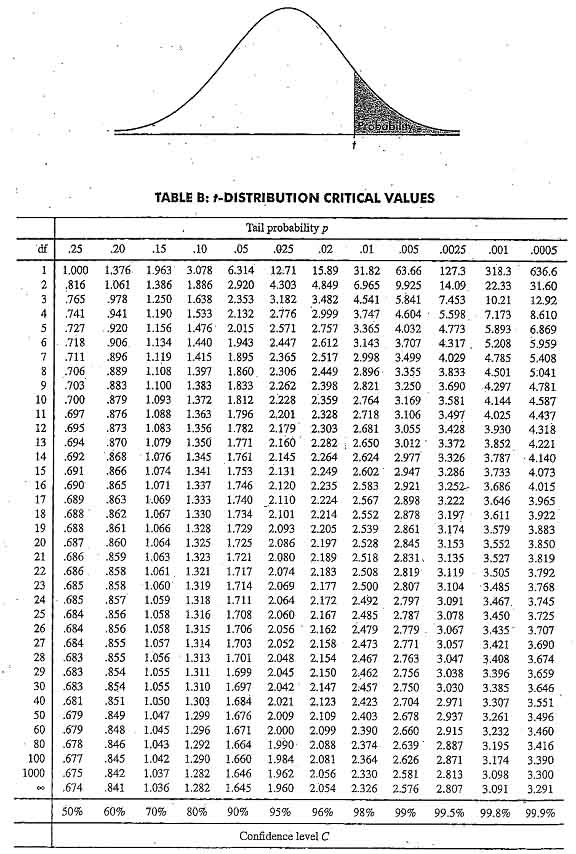
\includegraphics[width=1.1\linewidth]{gfx/t-table}
		\end{center}
	\caption[The T-Table]{The T-Table}
	\label{t_table}
	\end{figure}	


\section{Acknowledgement}
	I thank Mr. Vivek Sagar for helping me count the papillae on my tongue. I acknowledge the contribution of everyone in our section for performing the experiment.
	\par
	I am grateful to our Instructor, Prof. N. G. Prasad for the rest (which is statistically the most significant part anyway).

\section{References}
	\begin{enumerate}
		\item 	McMohan, K.A. 2008. Supertasters-Updating the taste test for the A and P laboratory. Pages 398-405, in Tasted Studies fro Laboratory Teaching, Volume 29 (K.L. Clase, Editor)
		\item \url{statstutorstl.blogspot.com} for the t-table.
	\end{enumerate}